%\VignetteIndexEntry{Tutorial on Bayesian 1-D and 2-D Genome Scans}
%\VignetteDepends{qtlbim}
%\VignetteKeywords{QTL}
%\VignettePackage{qtlbim}

\documentclass[12pt]{article}
\usepackage[margin=1in,head=0.5in,foot=0.5in]{geometry}



\usepackage{/unsup/R-2.4.0/lib/R/share/texmf/Sweave}
\begin{document}

\title{Tutorial on Bayesian 1-D and 2-D Genome Scans}
\author{Brian S. Yandell and W. Whipple Neely}
\maketitle
\newpage
\tableofcontents
\newpage
\abstract{We present an introduction to QTL analysis based on new 
Bayesian scan routines available in the {\tt R/qtlbim} package.  These 
routines allow exploration of single and multiple QTL models.  
Additionally plotting routines allow visual exploration of the genetic 
architecure for a phenotypic trait.  We present tutorial examples 
based on both experimental and simulated data.}

\section{Overview}
This document describes 1-D and 2-D Bayesian genome scan routines 
available in the {\tt R/qtlbim} package.  In the present context, the 
term ``scan'' refers to  methods based on constructing one or two 
dimensional profiles of QTL likelihoods or posterior distributions.  
These new scan routines  in {\tt R/qtlbim} are analogous to the 
routines {\tt scanone} and  {\tt scantwo} from  the {\tt R/qtl} 
package.  On a practical level, using {\tt R/qtlbim} scan routines is  
very similar to using {\tt R/qtl}'s  {\tt scanone} and {\tt scantwo} 
methods.   The key difference  between the  scan  routines in  
{\tt R/qtlbim} and the scan routines in {\tt R/qtl} lies in the 
technique used for  constructing QTL summaries.  {\tt R/qtlbim}  
extends {\tt R/qtl} by providing the ability to generate  Markov chain 
Monte Carlo (MCMC) samples from a posterior distribution for 
the genetic architecture of a trait.  Furthermore the putative genetic 
architectures sampled can include an arbirary number of QTL.  


The {\tt R/qtlbim} package's scan routines  are called  {\tt qb.scanone} 
and {\tt qb.scantwo}.  Because these scans are motivated by Bayesian 
MCMC techniques we refer to {\tt qb.scanone} and {\tt qb.scantwo} 
collectively as ``qb.scans'' or ``qb.scan routines''.    The utility of 
the qb.scan routines lies in their ability to provide interpretable 
summaries of the high-dimensional MCMC samples.  The scan summaries use 
ideas of Bayesian model  averaging to explore the most probable models 
given the data.  For example, in a one dimensional genome scan, we 
might consider the contribution of each potential locus averaging over 
all  sampled models that include  that locus. This allows us to  adjust 
for the possible effects of all other loci by examining the marginal  
distributions. This has the advantage of reducing variation explained 
by other loci and reducing bias due to  linked loci.  Thus a one 
dimensional marginal scan can be informative about higher-order models 
directly without bias or variance inflation.  Although the development 
of the {\tt qb.scan} routines is motivated by Bayesian techniques, the 
interpretation of qb.scans  involve a mix of frequentist and Bayesian 
ideas.  In what follows we show the  
resolving power of low-dimensional scans that condition on the presence 
of  other QTL using simulated data with  one QTL and the {\tt hyper} 
data set.


\section{Using and Interpreting Qb.Scan Routines}
This section illustrates the basic uses and interpretation of the qb.scan 
routines using simulated data and the {\tt hyper}  data included in
the {\tt R/qtl} package. In later  experimental data.  The value of
using simulated data is that we have complete control over the model
from which the data are generated, so that we can provide very simple
examples with predictable outcomes. We first attach the {\tt R/qtlbim}
library, which in turn attaches {\tt R/qtl} and other needed
libraries.
\begin{Schunk}
\begin{Sinput}
> library(qtlbim)
\end{Sinput}
\end{Schunk}

\subsection{Loading the {\tt hyper} Data}
The {\tt hyper} data come from 250 backcross individuals in which the 
phenotype is blood pressure. To load {\tt hyper} use the command
\begin{Schunk}
\begin{Sinput}
data(hyper)
\end{Sinput}
\end{Schunk}
A summary of {\tt hyper} can be displayed with 
\begin{Schunk}
\begin{Sinput}
> summary(hyper)
\end{Sinput}
\begin{Soutput}
    Backcross

    No. individuals:    250 

    No. phenotypes:     2 
    Percent phenotyped: 100 100 

    No. chromosomes:    19 
        Autosomes:      1 2 3 4 5 6 7 8 9 10 11 12 13 14 15 16 17 18 19 

    Total markers:      170 
    No. markers:        22 8 6 20 14 11 7 6 5 5 14 5 5 5 11 6 12 4 4 
    Percent genotyped:  47.9 
    Genotypes (%):      AA:50.1  AB:49.9 
\end{Soutput}
\end{Schunk}
We need to exclude the X chromosome from our work with {\tt hyper} as 
{\tt R/qtlbim} does not yet handle this properly.  To 
accomplish this we identify the chromosome named ``{\tt X}'' and select all 
but this chromosome.   
\begin{Schunk}
\begin{Sinput}
hyper <- subset(hyper,sapply(hyper$geno,class) != "X")
\end{Sinput}
\end{Schunk}

\subsection{Running the MCMC Analysis on Simulated Data \& 
The {\tt hyper} Data}
Now that we have data, we can begin to use the new methods available 
through {\tt R/qtlbim}. The next step in using the {\tt R/qtl} package 
would be to use the function {\tt calc.genoprob} to create  genotype 
probabilities based on a Hidden Markov model.  For the Bayesian model 
selection, we replace  {\tt calc.genoprob} with  the  {\tt R/qtlbim} 
function {\tt qb.genoprob} followed by the MCMC sampler 
({\tt qb.mcmc}).  The MCMC sampler has random number generator 
and does not use {\tt R}'s built-in random number generator, in order 
to make our simulations repeatable we pass an integer seed 
({\tt qb.random.seed}) directly to {\tt qb.mcmc}.  
By default the {\tt qb.mcmc} function prints out progress messages 
of the number of iterations completed.  These progress messages can be 
suppressed by setting {\tt verbose=FALSE}.  To run the MCMC sampler on 
the {\tt hyper} data we use the command
\begin{Schunk}
\begin{Sinput}
hyper <- qb.genoprob(hyper, step=2)
qb.random.seed <- 1616
qbHyper <- qb.mcmc(hyper, genoupdate=TRUE, n.iter = n.iter, 
  seed = qb.random.seed, verbose=FALSE,mydir="scanPDF")
\end{Sinput}
\end{Schunk}

\subsection{Using {\tt qb.scanone}}
The object {\tt qbHyper} created above contains the results of the MCMC 
run.  Each iteration of the Monte Carlo chain represents a single QTL 
model.  The entire Monte Carlo chain represents a sample from the 
posterior distribution of all possible models.  One simple summary of 
the MCMC sample is the posterior profile, or the
posterior probability of a QTL at each locus.  A summary and plot of
these counts is carried out as follows.
\begin{Schunk}
\begin{Sinput}
> temp <- qb.scanone(qbHyper, type = "posterior")
> summary(temp)
\end{Sinput}
\begin{Soutput}
posterior of bp for main,epistasis,sum 

     n.qtl   pos m.pos e.pos    main epistasis     sum
c1  1.3310 64.50 64.50 67.80 0.23309   0.03897 0.23501
c2  0.3477 51.90 51.90 42.63 0.01837   0.00651 0.02008
c3  0.1453 30.63 30.63  8.76 0.00443   0.00565 0.00663
c4  1.3770 29.50 29.50 29.50 0.71470   0.11669 0.71470
c5  0.2447 68.87 68.87 82.00 0.01944   0.01089 0.02151
c6  0.8383 59.00 59.00 59.00 0.17383   0.17390 0.18117
c7  0.1553 13.10 55.60 15.28 0.00249   0.01074 0.01122
c8  0.1320 56.93 59.00 17.52 0.00367   0.00501 0.00610
c9  0.1173 12.00 64.87 12.00 0.00305   0.00617 0.00645
c10 0.0947 37.95 75.40 37.95 0.00314   0.00342 0.00444
c11 0.1717 13.10 39.57 13.10 0.00368   0.00617 0.00709
c12 0.0947  1.10 46.55  1.10 0.00206   0.00547 0.00713
c13 0.0767 24.40 28.40 14.23 0.00215   0.00426 0.00462
c14 0.0840  0.00 46.35  0.00 0.00277   0.00414 0.00532
c15 0.9607 17.50 17.50 17.50 0.08125   0.15770 0.15887
c16 0.0813  8.37  8.37 10.46 0.00234   0.00377 0.00543
c17 0.1123 50.30 50.30 50.30 0.00186   0.00686 0.00743
c18 0.0663  2.20 14.20  2.20 0.00241   0.00670 0.00777
c19 0.1117 55.70 53.62 55.70 0.00487   0.00474 0.00760
\end{Soutput}
\end{Schunk}
\begin{figure}
\begin{Schunk}
\begin{Sinput}
> plot(temp)
\end{Sinput}
\end{Schunk}
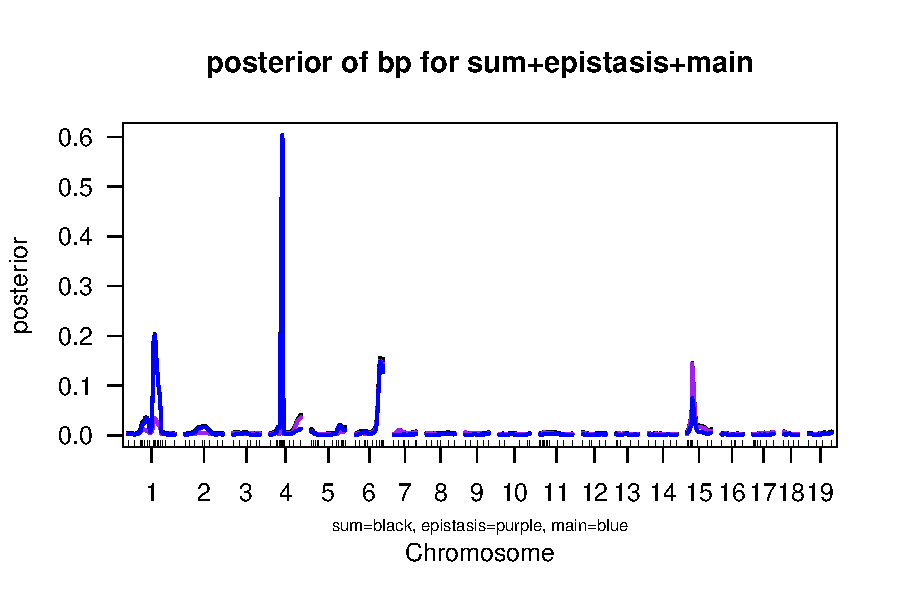
\includegraphics{scanPDF/FIG-Scanone-HyperPost}
\caption{Plot of {\tt qb.scanone} for posterior of simulated data.  Notice 
the posterior concentrated on chromosomes 1, 4, 6 and 15.}
\end{figure}
The plot shows the posterior concentrated on chromosomes 1, 4, 6 and
15. This is consistent with other findings for these data.
The blue lines in the plot indicate main effects, the 
purple indicate epistatic effects and black curves (where visible) 
represent the sum of main and epistatic effects.   

Here we show 2log(BF), or log of the Bayes factor,
measuring the strength of evidence (> 2.1 is high) for a QTL.
In order to examine the effects on 1, 4, 6 and 15 more closely, we can
plot subsets of chromosomes by using the plot 
command {\tt plot(temp, chr=c(1,4,6,15)}.  
\begin{Schunk}
\begin{Sinput}
> temp <- qb.scanone(qbHyper, type = "2logBF")
\end{Sinput}
\end{Schunk}
\begin{figure}
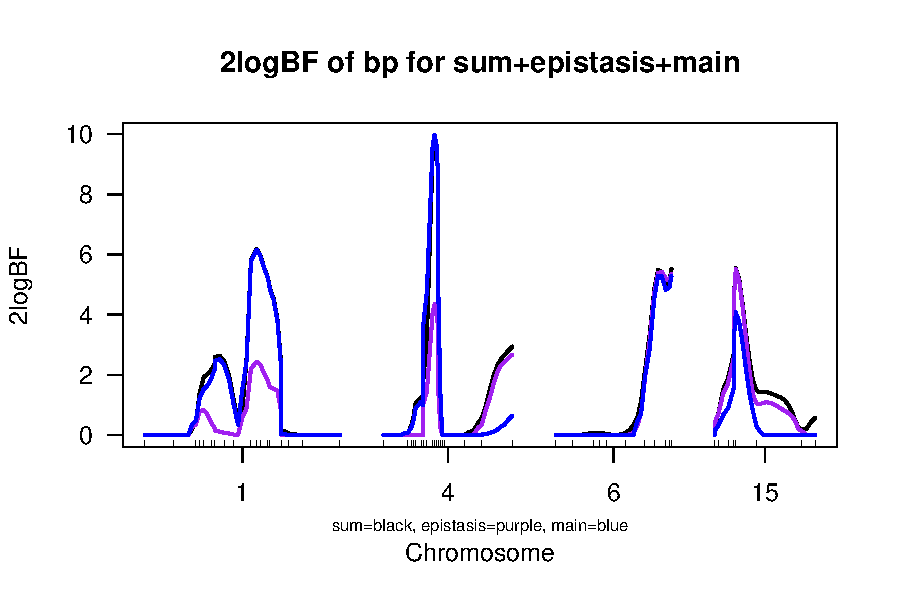
\includegraphics{scanPDF/FIG-Scanone-HyperSubset}
\caption{The {\tt qb.scanone} results for the {\tt hyper} data restricted 
to chomosomes 1,4,6 and 15.}
\label{fig-subsetsqb.scanone}
\end{figure}

\subsection{Using {\tt qb.scantwo}}
The function {\tt qb.scantwo} gives a two dimensional scan that allows us 
to look for possible epistatic effects between  putative QTL.   Before 
using {\tt qb.scantwo} on the {\tt hyper} data set we will illustrate the 
the use and interpretation of {\tt qb.scantwo} on extremely simple 
simulated data.  After examining the results from the simulated data we 
will use {\tt qb.scantwo} to explore the {\tt hyper} data set. 
 
\subsubsection{Simulating Data with Epistatic Effects \& No Main 
Effects}
In order to simulate data for which there is an epistatic effect but no 
main effects, we use the {\tt R/qtlbim} function {\tt
qb.sim.cross}. Through the rest of this document we {\it reuse} the
names of objects {\tt sim} and {\tt qbSim} to simplify presentation,
but their contents change depending on the example.
\begin{enumerate}
\item Determine the positions of qtl by specifying the 
 {\tt qtl.positions} parameter. This parameter gives a matrix with 
dimensions {\tt (number of qtl)} x 2.  Each row identifies a qtl, 
the first column's entries represent the chromosome's index, the second 
column's entries represent the location on the chromosome of the qtl.   
The order in which qtl are listed in this parameter is the  index by 
which they are identified later on in the parameters 
{\tt qtl.main} and {\tt qtl.epi}.
\begin{Schunk}
\begin{Sinput}
> qtl.positions <- rbind(qtl1 = c(chromosome = 1, 
+     locus = 5), qtl2 = c(chromosome = 1, locus = 50), 
+     qtl3 = c(chromosome = 2, locus = 33))
> qtl.positions
\end{Sinput}
\begin{Soutput}
     chromosome locus
qtl1          1     5
qtl2          1    50
qtl3          2    33
\end{Soutput}
\end{Schunk}
\item Specify the main effects of the qtl by the {\tt qtl.main.model} 
parameter. The qtl indices listed here are the row indices of the 
{\tt qtl.positions} (or {\tt qtl.pos}) parameter.
\begin{Schunk}
\begin{Sinput}
> qtl.main.model <- rbind(qtl1.main.effect = c(qtl = 1, 
+     main.effect.size = 0), qtl2.main.effect = c(qtl = 2, 
+     main.effect.size = 0), qtl3.main.effect = c(qtl = 3, 
+     main.effect.size = 0))
> qtl.main.model
\end{Sinput}
\begin{Soutput}
                 qtl main.effect.size
qtl1.main.effect   1                0
qtl2.main.effect   2                0
qtl3.main.effect   3                0
\end{Soutput}
\end{Schunk}
\item Specify the epistatic effects using the {\tt qtl.epi.model} 
parameter.
\begin{Schunk}
\begin{Sinput}
> qtl.epi.model <- rbind(qtl1.and.qtl3.epi.effect = c(qtl1 = 1, 
+     qtl2 = 3, epi.effect.size = 10))
> qtl.epi.model
\end{Sinput}
\begin{Soutput}
                         qtl1 qtl2 epi.effect.size
qtl1.and.qtl3.epi.effect    1    3              10
\end{Soutput}
\end{Schunk}
\item  Call the {\tt qb.sim.cross} function.   The parameter {\tt len} 
gives the lengths of each chromosome. Thus \texttt{len = c(80,90,44)} 
would represent a model with three  chromosomes of lengths 80, 90, and 
44 respectively.    Similarly the parameter {\tt n.mar} gives the 
number of markers on each chromosome.  If a single number is entered 
for {\tt n.mar} then all chromosomes will have the same number of 
markers.
\begin{Schunk}
\begin{Sinput}
set.seed(1234)
sim <- qb.sim.cross(len=rep(100,2), n.mar=10, eq.spacing=TRUE, 
  n.ind=100, type="bc", missing.geno=0.03, qtl.pos=qtl.positions, 
  qtl.main=qtl.main.model, qtl.epis=qtl.epi.model)
\end{Sinput}
\end{Schunk}
\end{enumerate}
Finally we can run {\tt qb.genoprob} and {\tt qb.mcmc} on the 
simulated data, just as we would for  data that arose from an actual 
experiment. 
\begin{Schunk}
\begin{Sinput}
## Call qb.genoprob to fill in missing data.
sim <- qb.genoprob(sim)
## Call qb.mcmc and then analysis code.
qbSim <- qb.mcmc(sim,n.iter=n.iter,verbose=FALSE,
                    seed=qb.random.seed,mydir="scanPDF")
\end{Sinput}
\end{Schunk}
Next we use qb.scantwo to examine the heritability, or percent
varianced explained, per pair of loci.
\begin{Schunk}
\begin{Sinput}
> temp <- qb.scantwo(qbSim)
> summary(temp, digits = 2)
\end{Sinput}
\begin{Soutput}
upper: heritability of pheno.normal for epistasis
lower: heritability of pheno.normal for full 

      n.qtl l.pos1 l.pos2 lower u.pos1 u.pos2 upper
c1:c1 1.353  57.78   68.9  18.9  46.67   88.9  16.2
c1:c2 2.976   2.22   26.7  85.5   2.22   24.4  85.6
c2:c2 0.738  60.00   77.8  23.9  60.00   77.8  23.9
\end{Soutput}
\end{Schunk}
\begin{figure}
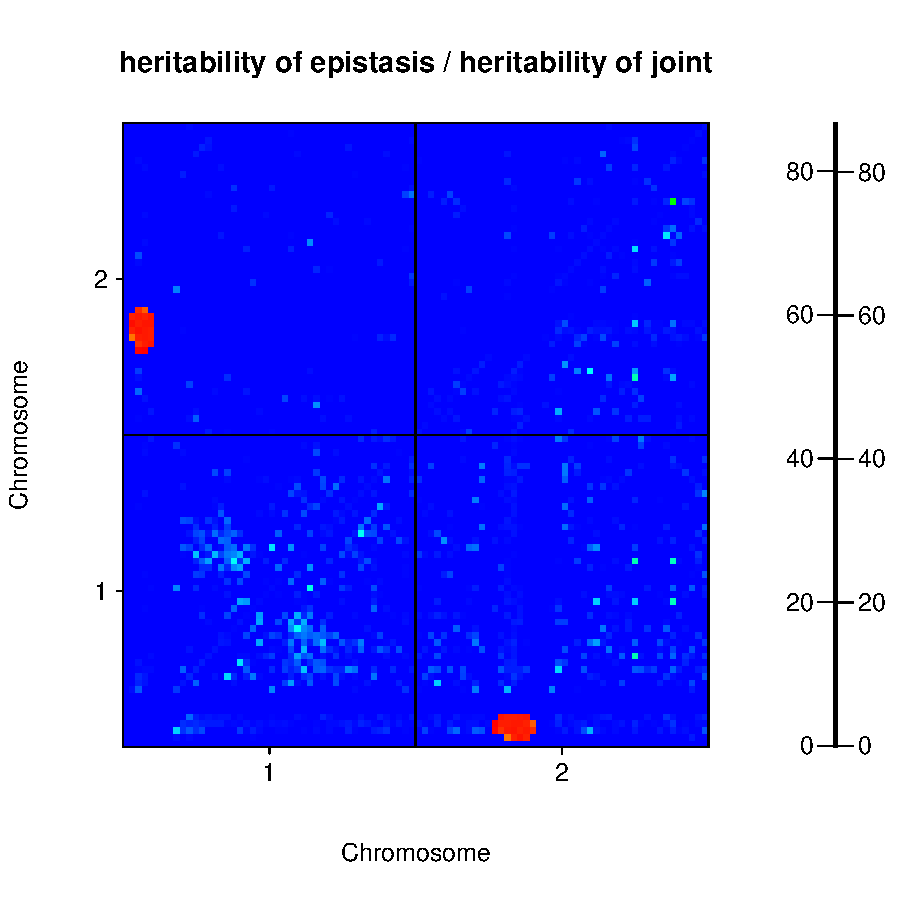
\includegraphics{scanPDF/FIG-Scantwo-SimEpi}
\caption{Plot of {\tt qb.scantwo} results from simulated data with an 
epistatic effect but no main effects.  Heritability is R-squared, or
percent variation explained. Epistasis in the upper triangle is
indicated by the two isolated peaks.  Notice that the peaks occur 
at  the locations expected from the simulation: around 5 {\tt cm} on 
chromosome one and 33 {\tt cm} on chromosome two.}
\end{figure}

\noindent
The plot of the results from running {\tt qb.scantwo} on the simulated 
data shows two isolated peaks each representing the  interaction of the 
first and third QTL.  This illustrates that under idealized 
circumstances we would expect a plot of {\tt qb.scantwo} results to show 
evidence for epistasis in the form of a peak in the vicinity of the 
position corresponding to the loci of the two QTL.

\subsubsection{Simulating Data with Main Effects But No Epistatic 
Effects.}
In order to illustrate the extreme case where there are main effects 
but no epistatic effects we can modify the simulation parameters 
{\tt qtl.main.model} and {\tt qtl.epi.model}.  Since 
{\tt qtl.main.model} consisted entirely of zeros (indicating no main 
effects), we can add a main effect of size 10 for the second QTL as 
follows.
\begin{Schunk}
\begin{Sinput}
> qtl.main.model[2, "main.effect.size"] = 10
\end{Sinput}
\end{Schunk}
Since we have no epistatic component to the new model, we replace 
{\tt qtl.epi.model} in the call to {\tt qb.sim.cross} with {\tt NULL}.
\begin{Schunk}
\begin{Sinput}
set.seed(1234)
sim <- qb.sim.cross(len=rep(100,2), n.mar=10, eq.spacing=TRUE, 
  n.ind=100, type="bc",
  missing.geno=0.03, qtl.pos=qtl.positions, 
  qtl.main=qtl.main.model, qtl.epis=NULL) 
\end{Sinput}
\end{Schunk}
Running {\tt qb.sim.cross}, {\tt qb.mcmc} and plotting the results of 
{\tt qb.scantwo} gives a plot of data in which there is no 
epistatic effect, but in which there is a main effect.  This is indicated
by the horizontal band near 50 {\tt cM} on chromosome 1.
\begin{Schunk}
\begin{Sinput}
sim <- qb.genoprob(sim)
qbSim <- qb.mcmc(sim,n.iter=n.iter,verbose=FALSE,
                   seed=qb.random.seed,mydir="scanPDF")
\end{Sinput}
\end{Schunk}
\begin{Schunk}
\begin{Sinput}
> temp <- qb.scantwo(qbSim)
> summary(temp, digits = 2)
\end{Sinput}
\begin{Soutput}
upper: heritability of pheno.normal for epistasis
lower: heritability of pheno.normal for full 

      n.qtl l.pos1 l.pos2 lower u.pos1 u.pos2 upper
c1:c1 0.983   55.6   80.0  96.7   73.3   84.4  12.7
c1:c2 1.179   53.3   11.1  96.4    0.0   35.6  10.3
c2:c2 0.295   51.1   66.7  12.1   75.6   84.4  12.9
\end{Soutput}
\end{Schunk}
\begin{figure}
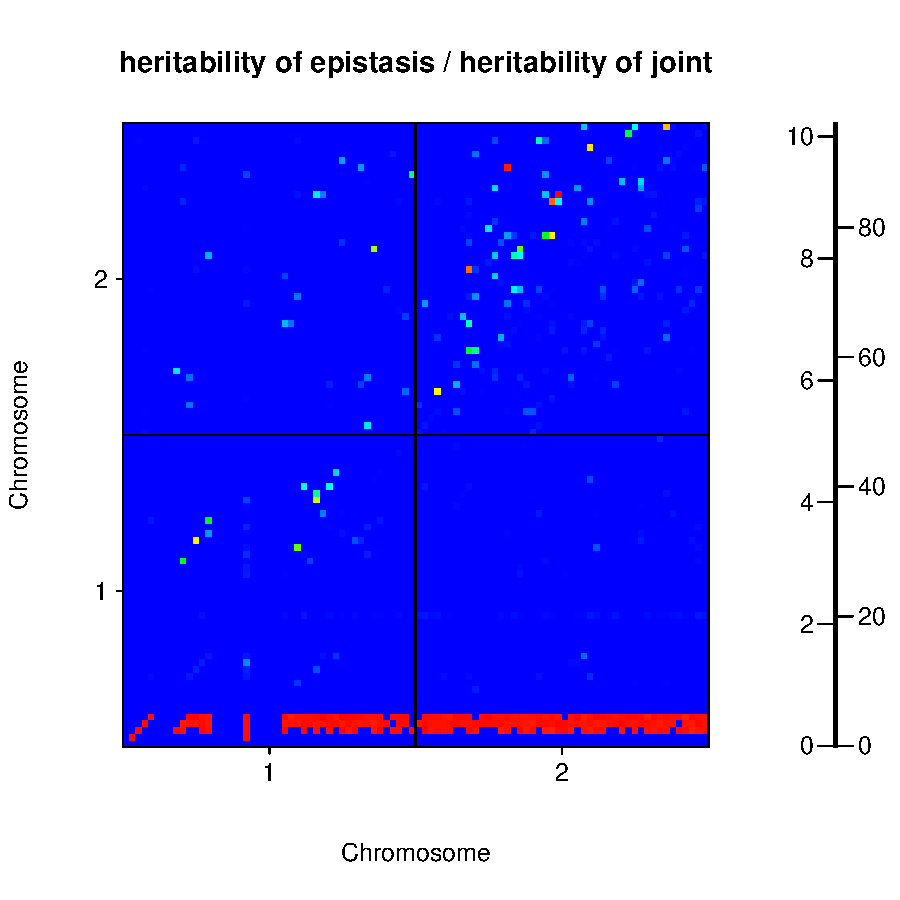
\includegraphics{scanPDF/FIG-Scantwo-SimMain}
\caption{The plot of \texttt{qb.scantwo} with a main effect for a QTL
at position 5 on chromosome 1 but no epistatic effect. Notice the long
band in the lower triangle.}
\label{fig-simnoepimain}
\end{figure}
Notice that in Figure~\ref{fig-simnoepimain} the main effect is
represented by the horizontal band at 5{\tt cm}. The corresponding
{\tt qb.scanone} results for {\tt qbSim} are shown in 
Figure~\ref{fig-simnoepimainscanone}.

\begin{figure}
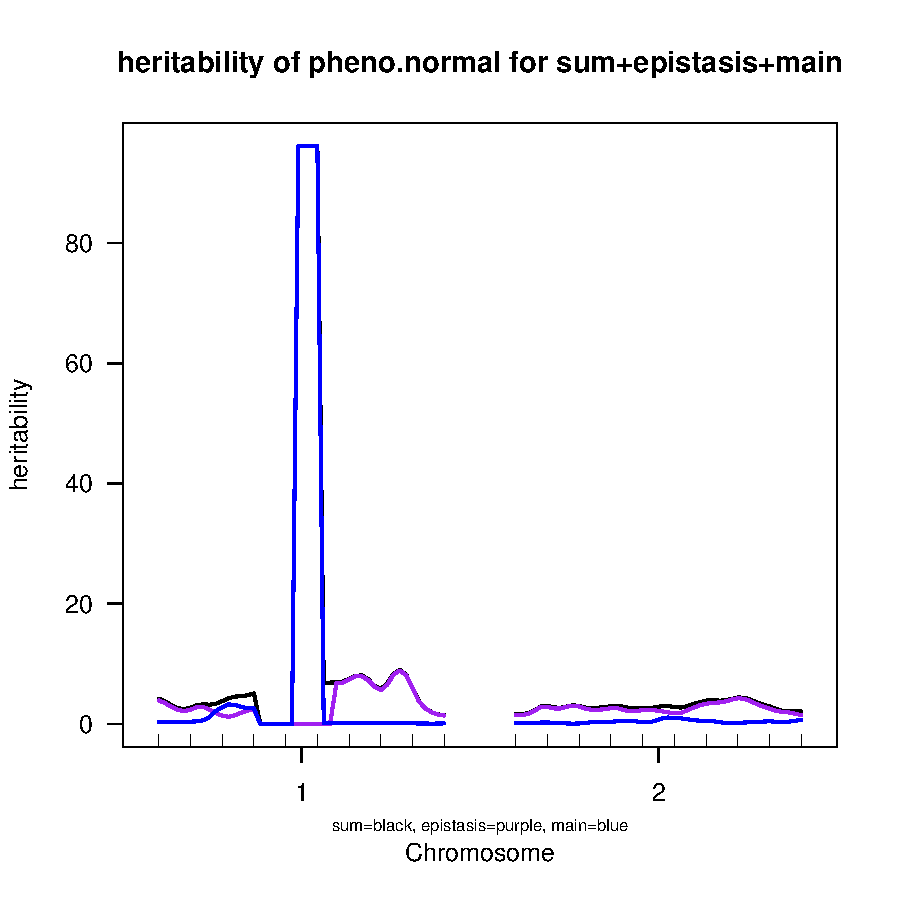
\includegraphics{scanPDF/FIG-Scanone-SimMainLog10}
\caption{Heritability for simulated data with main effect but no epistasis examined 
under {\tt qb.scanone}. As expected from the simulate there is a peak in the 
blue (main effects) curve near position five on chromosome one.}
\label{fig-simnoepimainscanone}
\end{figure}
 
\subsubsection{Simulating Data with Main Effects \& Epistatic Effects.}
As a final example of {\tt qb.scantwo} operating on simulated data, we 
can take a look at data that involves both an epistatic effect and a 
main effect.  We use the value of {\tt qtl.main.model} above, 
which specifies a main effect and the original value of 
{\tt qtl.epi.model}.
\begin{Schunk}
\begin{Sinput}
set.seed(1234)
sim <- qb.sim.cross(len=rep(100,2), n.mar=10, eq.spacing=TRUE, 
  n.ind=100, type="bc", missing.geno=0.03, qtl.pos=qtl.positions, 
  qtl.main=qtl.main.model, qtl.epis=qtl.epi.model) 
\end{Sinput}
\end{Schunk}
Running {\tt qb.sim.cross}, {\tt qb.mcmc} and plotting the results of 
{\tt qb.scantwo} gives an idealized plot of data with both main and
epistatic effects. It is essentially an overlay of the previous two
plots. We leave the details to the reader.

\subsubsection{Running {\tt qb.scantwo} on the {\tt hyper} Data}
To run qb.scan two on the hyper data set, we can use our previous results 
of the MCMC algorithm running on the {\tt hyper} data. 
\begin{Schunk}
\begin{Sinput}
> temp <- qb.scantwo(qbHyper, chr = c(4, 6, 15))
> summary(temp, digits = 2)
\end{Sinput}
\begin{Soutput}
upper: heritability of bp for epistasis
lower: heritability of bp for full 

        n.qtl l.pos1 l.pos2 lower u.pos1 u.pos2 upper
c4 :c4  0.261   16.4   18.6 23.65  54.35   65.6  6.22
c4 :c6  1.452   29.5   59.0 24.28  72.11   25.1  8.08
c4 :c15 0.417   21.9   63.4 23.02  14.20   41.6 10.67
c6 :c6  1.185    0.0   49.2 11.37   7.35   49.2  1.55
c6 :c15 1.004   59.0   17.5 17.82  59.00   19.5 10.25
c15:c15 0.111    7.7   13.1  5.68  23.50   27.5  5.05
\end{Soutput}
\end{Schunk}
\begin{figure}
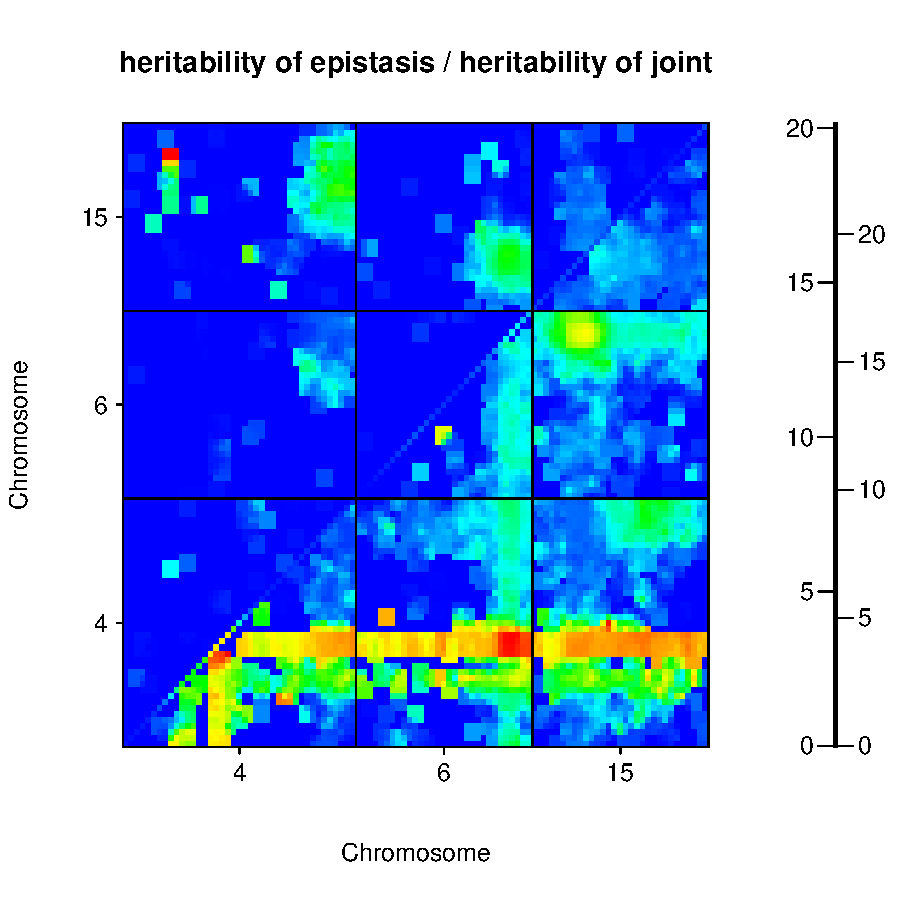
\includegraphics{scanPDF/FIG-Scantwo-HyperData}
\caption{A plot of a {\tt qb.scantwo} scan of the {\tt hyper} data 
showing results for chromosomes 1, 4,6, and 15. Note the main effect from 
the QTL on chromosome 4 and the epistatic effect between the pairs of 
QTLs on  chromosomes 4 and 15 and 6 and 15.}
\end{figure}
Using the results from the two-dimensional qb.scans of the simple 
simulated data as a guide, the plot of {\tt qb.scantwo} shows a 
main effect from a QTL on chromosome 4 and epistatic
effects between the pairs of QTLs on chromosomes 4 and 15 and 6 and 15. 

\section{Types of Scan Summaries}

We have created several types of scan summaries, illustrated
below. These include the following LPD, heritability, variance
components, parameter estimates, cell means, posterior probabilities
and Bayes factors. Below we detail what these are and how they are
calculated.

For each type, we can provide a summary scan, and in addition provide
detail broken down by main effects, epistatic effects, and/or GxE
(genotype by environment, or genotype by covariate)
interactions. These breakdowns can be further divided into Cockerham
(1954; see Kao and Zeng 2002) type effects (additive and dominance for
main effects, or the four epistatic interactions of aa, ad, da, dd) if
desired.

\begin{itemize}
\item
{\tt count} gives the count of the number of MCMC samples including
this locus. Currently this can be viewed on a log scale using type
{\tt log10}.
\item
{\tt posterior} is the Bayesian posterior probability, basically the
{\tt count} divided by the total number of MCMC samples.
\item
{\tt BF} provides the Bayes factor comparing the model with and
without this locus. It is more easily viewed as {\tt 2logBF}.
\item
{\tt estimate} gives model parameter estimates for main effects,
epistasis, and GxE interactions.
\item
{\tt cellmean} provides marginal means at a locus, adjusted for all
other model effects from other QTL and covariates.
\item
{\tt variance} yields the variance components for QTL effects
associated with a particular locus.
\item
{\tt heritability} is actually at this point explained variation. In a
future release we may distinguish Rsquared and idealized
heritability.
\item
{\tt LPD} is the log posterior density, adapted from Morton's (1995)
log odds ratio (LOD) used in human genetics to LOD maps by Lander and
Botstein (1989). The LPD for QTLs was introduced by Sen and Churchill
(2001). It tests presence or absence of a QTL at a locus, adjusting
for all other possible model effects (other QTL, epistasis and
GxE). The {\tt LPD}, the {\tt LR} or likelihood ratio, and the {\tt
deviance} are detailed in the next section.
\item
{\tt detection} is the posterior probability of detection of a QTL at
a locus.
\end{itemize}

\section{Theoretical Development}

This section could be skipped. It is aimed at those quantitative folks
who have read Yi et al. (2005) for the math and want to know
more. Here we leave out details concerning covariates to simplify
presentation.

Given complete data on genotypes for all individuals across the
genome, we could consider a model relating phenotype $y$ to genotype
$g$ through a design matrix $X$,
$$
y = \mu + X\Gamma\beta + e~.
$$
The unknown effect parameters are the grand mean, $\mu$, the
effect parameters, $\beta$, and the unexplained variance, $\sigma^2 =
V(e)$, which for convenience, we bring together as 
$\theta = (\mu, \beta, \sigma^2)$\,.
The genetic architecture is specified by 
$\Gamma = \mbox{diag}\gamma$, which has values of 1 or 0 to indicate
presence or absence, respectively, of the corresponding model
effect. The QTL model could thus be written as 
$p(y\vert \gamma, X, \theta)\,$.

This genetic architecture specified by a 0-1 vector $\gamma$ allows us
to consider models of different dimensions, e.g. one vs. two QTL,
without resorting to a more complicated (reversible jump) sampling
scheme. The unknown values $\gamma$ are the key device in
sampling over many different possible genetic architectures, in terms
of what loci $\lambda$ are included and what gene action is
important. There is some redundancy between $\gamma$ and $\lambda$: a
locus is in the model only if at least one $\gamma$ associated with
that locus is 1. Technically, we consider probabilities 
$p(\lambda\vert\gamma)$
that can only be 0 or 1 to indicate whether the loci, $\lambda$\,, are
compatible with the genetic architecture, $\gamma$\,. While the loci
are determined by the genetic architecture, $\gamma$ is not completely
determined by $\lambda$. We exploit this to make more efficient code
and to build diagnostic summaries.

Recall from Yi et al. (2005) that the whole-genome genotype
information, $g$, and the design matrix, $X$, are 1-1 mappings. In
other words, $p(X\vert g)$ is either 0 or 1, depending on whether, for
instance, the design is compatible with the genotypes.

\subsection{Likelihood and posterior}

In a classical setting, the full likelihood augmented by genotypes,
$g$, over the genome is
$$
p(y,g\vert m, \gamma, \theta) =
p(y\vert \gamma, X, \theta)p(X\vert g)
p(g\vert m, \lambda)p(\lambda\vert\gamma)\,,
$$
with $m$ the marker genotypes across the genome and
$p(g\vert m, \lambda)$ the map function. At most loci, we do not fully
know genotypes $g$, hence the likelihood given observable data is
averaged over $g$,
$$
L(\gamma,\theta\vert y,m) =
\sum_g p(y,g\vert m, \gamma, \theta)\,.
$$
With no QTL, we write $L(\mu\vert y)$ for the null likelihood.

In a Bayesian perspective, a prior $p(\gamma,\theta)$ is placed on
the unknowns, and we study the posterior,
$$
p(g,\gamma, \theta\vert y,m ) \propto
p(y,g\vert m, \gamma, \theta)p(\gamma,\theta)\,.
$$
To study the unknown parameters of interest, $(\gamma, \theta)$\,, we
average the posterior over the genotypes, or equivalently, form a
weighted average of the augmented likelihood with weights proportional
to the prior on $(\gamma, \theta)$\,,
$$
p(\gamma, \theta\vert y,m ) = \sum_g p(g,\gamma, \theta\vert y,m )
\propto
\sum_g p(y,g\vert m, \gamma, \theta)p(\gamma,\theta)\,.
$$

\subsection{Parameter estimation}

Classically, the parameters of interest, $(\lambda, \theta)$\,, are
estimated by maximizing the likelihood. This is usually done in a QTL
setting by profiling the likelihood, or LOD (see below), with respect
to one locus or two loci over the genome. We think of that here as
profiling with respect to a given genetic architecture, $\gamma$\,, to
find the maximum likelihood estimate (MLE) for $\beta$ \,,
$$
\hat{\beta} = V\Gamma X^T y\,,
$$
with $V = (\Gamma X^T X \Gamma)^{-1}$ and $\sigma^2V$ the
variance-covariance matrix for $\hat{\beta}$\,. Here we assume the
columns of $X$ are centered on zero, so the MLE for the reference is
$\hat{\mu} = \bar{y}$\,.

Bayesian parameter estimates are typically found as the posterior
means, which shrink $\hat{\mu}$ toward its prior mean $\mu_0$ and
$\hat{\beta}$ toward the prior mean of 0, leading to posteriors
$$
\mu\sim N\left((1-b)\mu_0 +b\bar{y}, b\sigma^2/n.ind\right)~,
$$
and
$$
\beta\sim N\left(B\hat{\beta}, B\sigma^2V\right)~,
$$
with $b$ and $B$ being Bayesian shrinkage factors.  As we 
gather more data, the Bayesian priors focus on the MLEs, i.e. $b$ and
$B$ tend to 1. The likelihood and the posterior are both
fairly symmetric around the maximum, for any given $\gamma$. Thus, the
posterior mean and the MLE for $\beta$ are
very close in practice. This is less apparent from the summaries in
the previous section, as the Bayesian estimates are attenuated by the
putative effects of other QTL along the genome. This is a technical
post-processing issue of properly sorting out the effects of multiple
linked loci.

\subsection{Variance components}

Variance components can also be estimated in both approaches. The
classical unbiased estimate for environmental variance is
$\hat{\sigma}^2=RSS(\hat{\theta})/df$\,, with 
$RSS(\theta)=\sum(y-\mu-X\Gamma\beta)^2$ and 
$df = n.ind - 1 - \sum\gamma$.
%was found in the previous section to be
%$\ Sexpr{signif(summary(sim.scan)$sigma, 3)}^2 =
%\ Sexpr{signif(summary(sim.scan)$sigma^2, 3)}$
%for this simulation using R/qtl {\tt scanone}.

A Bayesian posterior estimate of $\sigma^2$ is its posterior mean,
which is a weighted average of $RSS(\theta)/n.ind$ and its prior mean. Its
empirical estimate can be found by averaging the posterior samples,

\begin{Schunk}
\begin{Sinput}
> summary(qb.scanone(qbSim, type = "variance", scan = "env"))
\end{Sinput}
\begin{Soutput}
variance of pheno.normal for env 

   n.qtl  pos m.pos   env
c1 1.666 46.7  46.7 0.940
c2 0.611 28.9  53.3 0.917
\end{Soutput}
\end{Schunk}

Heritability is computed as the percent of explained variation,
$h^2 = 100 (TSS-RSS(\theta))/TSS$\,,
with $TSS=\sum(y-\bar{y})^2$ the total sum of squares.
[The idealized variation would substitute expected fractions for the
$X^2$ terms based on the type of cross.] We can find the posterior
estimate of variability as the {\tt main} entry below:

\begin{Schunk}
\begin{Sinput}
> summary(qb.scanone(qbSim, type = "heritability"))
\end{Sinput}
\begin{Soutput}
heritability of pheno.normal for main,epistasis,sum 

   n.qtl  pos m.pos e.pos  main epistasis  sum
c1 1.666 46.7  46.7  64.4 96.13      6.93 96.1
c2 0.611 28.9  53.3  28.9  1.10      2.35  2.7
\end{Soutput}
\end{Schunk}

\subsection{LOD, LPD and BF}

The classical approach introduced by Lander and Botstein (1989)
profiles the likelihood only along the ridge 
of maximum $\beta$ for each $\lambda$. That is, at each $\lambda$,
find $\beta$ that maximizes the LOD. The LOD map is a plot of this
profile. The LOD statistic to assess QTL is
$$
LOD(\lambda) = c + \log_{10}
\left(
\max_{\theta} L(\gamma,\theta\vert y,m)p(\lambda\vert\gamma)
\right)\,,
$$
with the constant being $c=-\log_{10}(\max_{\mu} L(\mu\vert y))$\,.
The likelihood ratio is $LR=10^{LOD}$\,, and deviance is 
$D=2\log(10)LOD$\,.


The Bayesian approach provides a direct estimate of the posterior as
the histogram of the samples from the Markov chain Monte Carlo. Sen
and Churchill (2002) proposed profiling the log posterior 
density, LPD, which involves averaging over the unknown parameters
$\theta$,
$$
LPD(\lambda) = C + \log_{10}
\left(
\sum_{\theta} p(\gamma, \theta\vert y,m )p(\lambda\vert\gamma)
\right)\,.
$$
[The sum over $\theta$ is actually an multidimensional integral, but
we ignore those details here.]
Here the constant $C$ would involve averaging over the null likelihood
with respect to the prior on $\mu$. In practice, LOD and LPD are often
pretty close to each other and can be used interchangeably.

One advantage of sampling a large set of possible models by MCMC is
that Bayes factors are easily computed. We do not have to resort to
fancy harmonic means as in Newton and Raftery (199x). Instead, we
construct marginal posterior histograms for models to be compared, and
rescale by their priors. For instance, to compare two genetic
architectures, we construct
$$
BF = \frac{\displaystyle p(\gamma\vert y,m)/p(\gamma)}
{\displaystyle p(0\vert y)/p(0)}~,
$$
in which $p(0)$ is the prior on $\gamma$ being all zero (no QTL at
all) and $p(0\vert y)$ is the posterior. Actually,
$p(0\vert y)/p(0)\propto p(y)=\sum_{\mu}p(y\vert\mu)p(\mu)$\,,
with the sum really an integral over the real line.
Often this is more interpretable on a log scale as $2\log(BF)$\,,
which we can compute as

\begin{Schunk}
\begin{Sinput}
> summary(qb.scanone(qbSim, type = "2logBF"))
\end{Sinput}
\begin{Soutput}
2logBF of pheno.normal for main,epistasis,sum 

   n.qtl  pos m.pos e.pos main epistasis  sum
c1 1.666 46.7  46.7  64.4 5.58         0 5.58
c2 0.611 28.9  53.3  28.9 0.00         0 0.00
\end{Soutput}
\end{Schunk}

\subsection{Marginal Summaries}

Our primary interest here is in marginal statistics. Consider that the
model has genetic architecture $\gamma$ that include loci
$\lambda$\,. We want to ask what is the contribution to the model of
some subset of indicators, $\gamma_2$\,, associated with a locus, or a
set of loci, $\lambda_2$\,. We might ask this in a variety of ways,
looking at evidence in terms of LOD or a related statistics, or the
contribution in terms of variance components, heritability, or
parameter effects. We can think of partitioning the genetic
architecture into two components, $\gamma=(\gamma_1,\gamma_2)$\,,
with a corresponding partition of the effect parameters,
$$
\Gamma\beta=(\Gamma_1 + \Gamma_2)\beta~.
$$
The subset of effect parameters, $\beta_2=\Gamma_2\beta$\,, may
include, for instance, the main effects for locus $\lambda_2$ plus
some or all epistatic effects that involve this locus. We can then ask
questions about $\beta_2$, or about $\gamma_2$ and $\lambda_2$,
adjusting for the presence of effects $\beta_1=\Gamma_1\beta$\,. Note 
that $\beta_1$ could include some model parameters for $\lambda_2$.

\subsubsection{Variance components}

Here and through the rest of this document, we argue that we can
characterize important diagnostic summaries using marginal properties
of MCMC samples. The key technical argument is in the next
paragraph. Namely, we can use the marginal variance components of our
model fit, ignoring covariances, to construct approximate statistics.

If the columns of $X$ are nearly orthogonal to each other, then
the variance-covariance matrix for the effect parameter MLEs,
$\mbox{var}(\hat{\beta}) = \sigma^2V$\,,
would be {\em diagonally dominant}. That is, we suppose the variances
along the diagonal are larger than the sum of the absolute
covariances. Formally, with
$v=\mbox{diag}(V)$ and $V_{(j)}$ the $j$ column of $V$\,,
$$
2v_{(j)} \geq \sum \vert V_{(j)}\vert~.
$$

In other words, we assume the covariances among effect estimates are
negligible, and the diagonal values are approximately
$v_{(j)}\approx\gamma_{(j)}/\sum X_{(j)}^2$\,,
with $X_{(j)}$ the $j$th column of $X$\,.
In this case we can approximate $V$ by its diagonal, $D=\mbox{diag}(v)$,
and get a good approximation of $V^{-1}$ using $D^{-1}$:
$$
V^{-1}=D^{-1}[I+O]^{-1}~,
$$
with $O$ being on the order of $(V-D)D^{-1}$\,. As long as the
diagonal entries of $D$ are large, then this approximation
is good. Where these variances are small, the approximation is not so
useful. 

Since we are interested in learning about effects with larger
variance components, this approximation seems quite workable in the
present setting. It should a pretty reasonable between terms for
unlinked loci, and under conditions of Hardy-Weinberg equilibrium
among alleles at each locus. Note also that epistatic effects between
linked loci will be addressed directly by construction of columns of
$X$. 
[I believe the discrepancy of the diagonal can be readily checked
under H-W by adding another {\tt type} to the {\tt qb.scan}
routines--next freeze.] 

With this approximation the explained variation can be approximated as
$$
TSS-RSS(\theta)=\sum(X\Gamma\beta)^2 \approx \gamma^T r\,,
$$
with $r_{(j)}=\beta_{(j)}^2\sum X_{(j)}^2$ being the variance
explained by the $j$th component of the genetic architecture.
Then the difference, 
$RSS(\theta_1)-RSS(\theta) \approx \gamma_2^T r=\sum r_2$\,,
is simply the sum of variance components, which are readily stored for
each MCMC iteration. Here, $r_2$ contains the elements of $r$
corresponding to $\gamma_2 = 1$, and
$\theta_1=(\mu,\beta_1,\sigma^2)$\,.

Marginal heritability is computed as the additional variation
explained by the genetic architecture $\gamma_2$ given $\gamma_1$\,,
$$
h^2 = 
\frac{\displaystyle RSS(\theta_1) - RSS(\theta)}
{TSS}
=
\frac{\displaystyle \gamma_2^T r}
{TSS}
~.
$$

\subsubsection{LOD, LPD and BF}

The adjusted LOD to compare the full model to the reduced model with
$\gamma_2=0$ is
$$
LOD(\gamma_2\vert\gamma_1) = \log_{10} \left(
\frac{\displaystyle \max_{\theta} L(\gamma,\theta\vert y,m)}
{\displaystyle \max_{\theta_1} L(\gamma_1,\theta_1\vert y,m)}
\right)\,.
$$
The adjusted LPD is similarly,
$$
LPD(\gamma_2\vert\gamma_1) = \log_{10} \left(
\sum_{\theta}\frac{\displaystyle  p(\gamma,\theta\vert y,m)}
{\displaystyle p(\gamma_1,\theta_1\vert y,m)}
\right)\,,
$$
with again the sum actually being an integral over $\theta$\,.

In the case of normal data
and complete marker information, the LOD reduces to
$$
LOD(\gamma_2\vert\gamma_1) = \frac{n.ind}{2}
\log_{10} \left(
\frac{\displaystyle \min_{\theta_1} RSS(\theta_1)/df_1}
{\displaystyle \min_{\theta} RSS(\theta)/df}
\right)\,,
$$
with degrees of freedom, 
$df = n.ind - 1 - \sum\gamma$\,, and
$df_1 = n.ind - 1 - \sum\gamma_1$\,. The LPD follows a similar form,
but involving an average (or really, integral) over $\theta$\,,
$$
LPD(\gamma_2\vert\gamma_1) = \frac{n.ind}{2}
\log_{10} \left(
\sum_{\theta}
\frac{\displaystyle RSS(\theta_1)/df_1}
{\displaystyle RSS(\theta)/df}
\right)\,.
$$

The Bayes factors are easily computed, as noted earlier. To compare
the two genetic architectures $\gamma$ and $\gamma_1$\,, we construct
$$
BF = \frac{\displaystyle p(\gamma\vert y,m)/p(\gamma)}
{\displaystyle p(\gamma_1\vert y,m)/p(\gamma_1)}~.
$$
Often this is more interpretable on a log scale as $2\log(BF)$\,,
which we can compute as

\subsection{Model Averaging Algorithm}

Here we briefly describe the model averaging idea. The MCMC samples
include a wide variety of models, indexed by $\gamma$. The 1-D and 2-D
scans first compile a selected diagnostic for each sample (also known
as an iteration). That is, at each genome position, or pair of
positions, we average the values for samples that include that
position, i.e. have $\gamma=1$ at that position. The posterior is
simply an average of the $\gamma$ samples at each position.

These samples are kept for each model component, either in terms of
the un-aggregated Cockerham (1954) partition or in terms of {\tt main}
effects and {\tt epistasis}, and for the {\tt sum} of these
components. There are some mechanics involved. For instance, for 
1-D averages involving epistasis, we want to count each pair for both
loci, and for 2-D averages, we want to count epistatic effects
separately at each locus. But these are details that can be found by
looking at the code if interested.

Chromosome summaries, or summaries within regions of chromosomes, are
found as weighted averages of these per-position summaries. The
weights are naturally the number of MCMC samples per position. At
present the code does not separate out multiple loci on a chromosome
[next freeze].

With small or moderate MCMC sample sizes, the 1-D and 2-D scans can be
rather rough, or jagged. We have found nearest neighbor smoothing to
be helpful. That is, a position is equally weighted against the sum of
its neighbors, accounting for number of MCMC samples. This can be
repeated several times (e.g. {\tt smooth = 3}) to further local
smoothing. 

\section{Summary}
In this tutorial we have explored the use of the Bayesian scan routines 
{\tt qb.scanone} and {\tt qb.scantwo} as techniques for exploring the
genetic architecture for a phenotypic trait.  Through examples using 
both simulated and experimental data we have demonstrated the key steps in
identifying both main and epistatic effects.  Further information on using 
using {\tt R/qtlbim} to explore the {\tt hyper} data set can be found in the 
{\it hyperpaper} vignette.  Inorder to view the vignette you can simply type
\begin{Schunk}
\begin{Sinput}
vignette(topic="hyperpaper",package="qtlbim")
\end{Sinput}
\end{Schunk}
at the R prompt.
A demo for a simple analysis of {\tt hyper} can be accessed by typing 
{\tt demo(qb.hyper.tour)} after the {\tt R/qtlbim} library has been loaded.  

\begin{Schunk}
\begin{Soutput}
[1] TRUE
\end{Soutput}
\end{Schunk}

\section*{References}

Cockerham CC (1954) An extension of the concept of partitioning
hereditary variance for analysis of covariances among relatives when
epistasis is present. Genetics 39: 859-882. 

Kao CH, Zeng ZB (2002) Modeling epistasis of quantitative trait loci
using Cockerham's model. Genetics 160: 1243-1261.

Morton NE (1995) LODs past and present. Genetics 140: 7-12.

Newton MA, Raftery AE (1994) Approximate Bayesian inference by the
weighted likelihood bootstrap (with Discussion). Journal of the Royal
Statistical Society, series B, 56, 3-48.

Sen S, Churchill GA (2001) A statistical framework for quantitative
trait mapping. Genetics 159: 371-387. 

Sugiyama F, Churchill GA, Higgens DC, Johns C, Makaritsis KP, Gavras
H, Paigen B (2001) Concordance of murine quantitative trait loci for
salt-induced hypertension with rat and human loci. Genomics 71: 70-77.

Wright FA, Kong A (1997) Linkage mapping in experimental crosses: the
robustness of single-gene models. Genetics 146: 417-425. 

\end{document}
